\section{Video management overview}
\label{sec:Video_management_overview}

The use case of the thesis project, X-Learning, represents a platform in which the administrator or whichever authorized collaborator can manage the insert, the modifications and eliminations of the various courses.
Each course is characterized by a title, description, cost, teaching material, lessons and webinar.

\subsection{Course management}
\label{sec:course_management}

The course creation is articulated in two main phases:

\begin{itemize}
\item The first phase includes information such as title, description, language, cost, category, objectives and requirements needed to understand the content. Once the course is created, the first phase can be considered completed.
Subsequently the teacher will begin the second phase, which consists of adding video lectures and educational content.

\begin{figure}[htb]
 \centering
 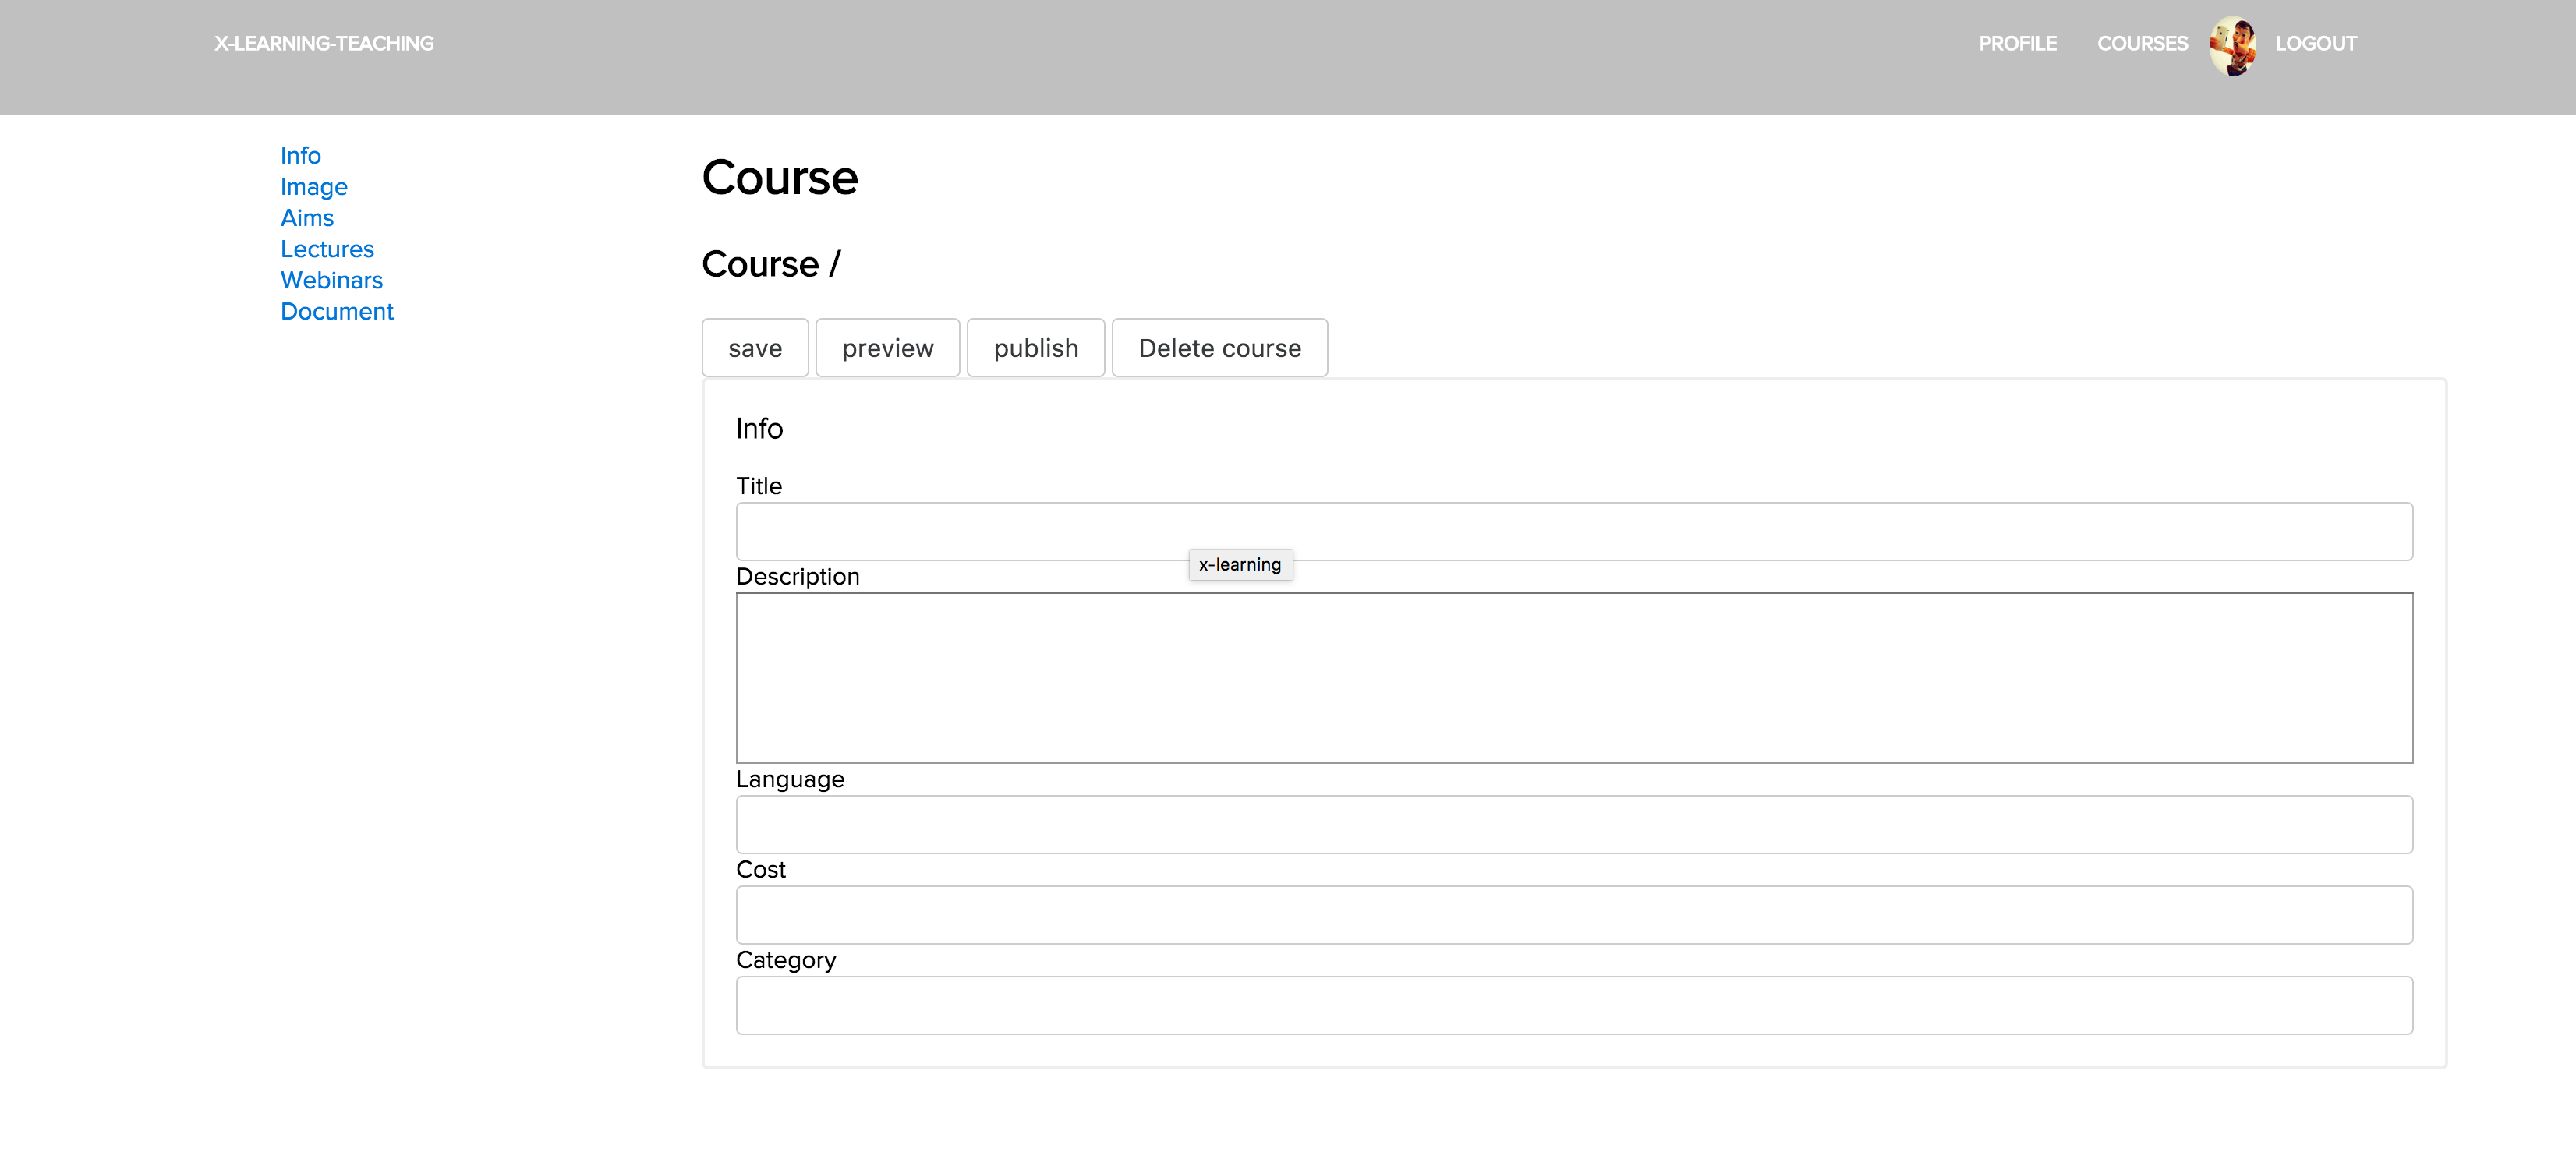
\includegraphics[width=1.0\linewidth]{images/chapter6/insert_course_page.png}\hfill
 \caption[Admin page course]{Admin page course}
 \label{fig:fourV}
\end{figure}

\item The second phase begins with the creation of the lectures, each of which will have a title, a description, and multimedia content.
The page displayed in the picture allows the teacher to select the video that will be associated with the current lesson.

\begin{figure}[htb]
 \centering
 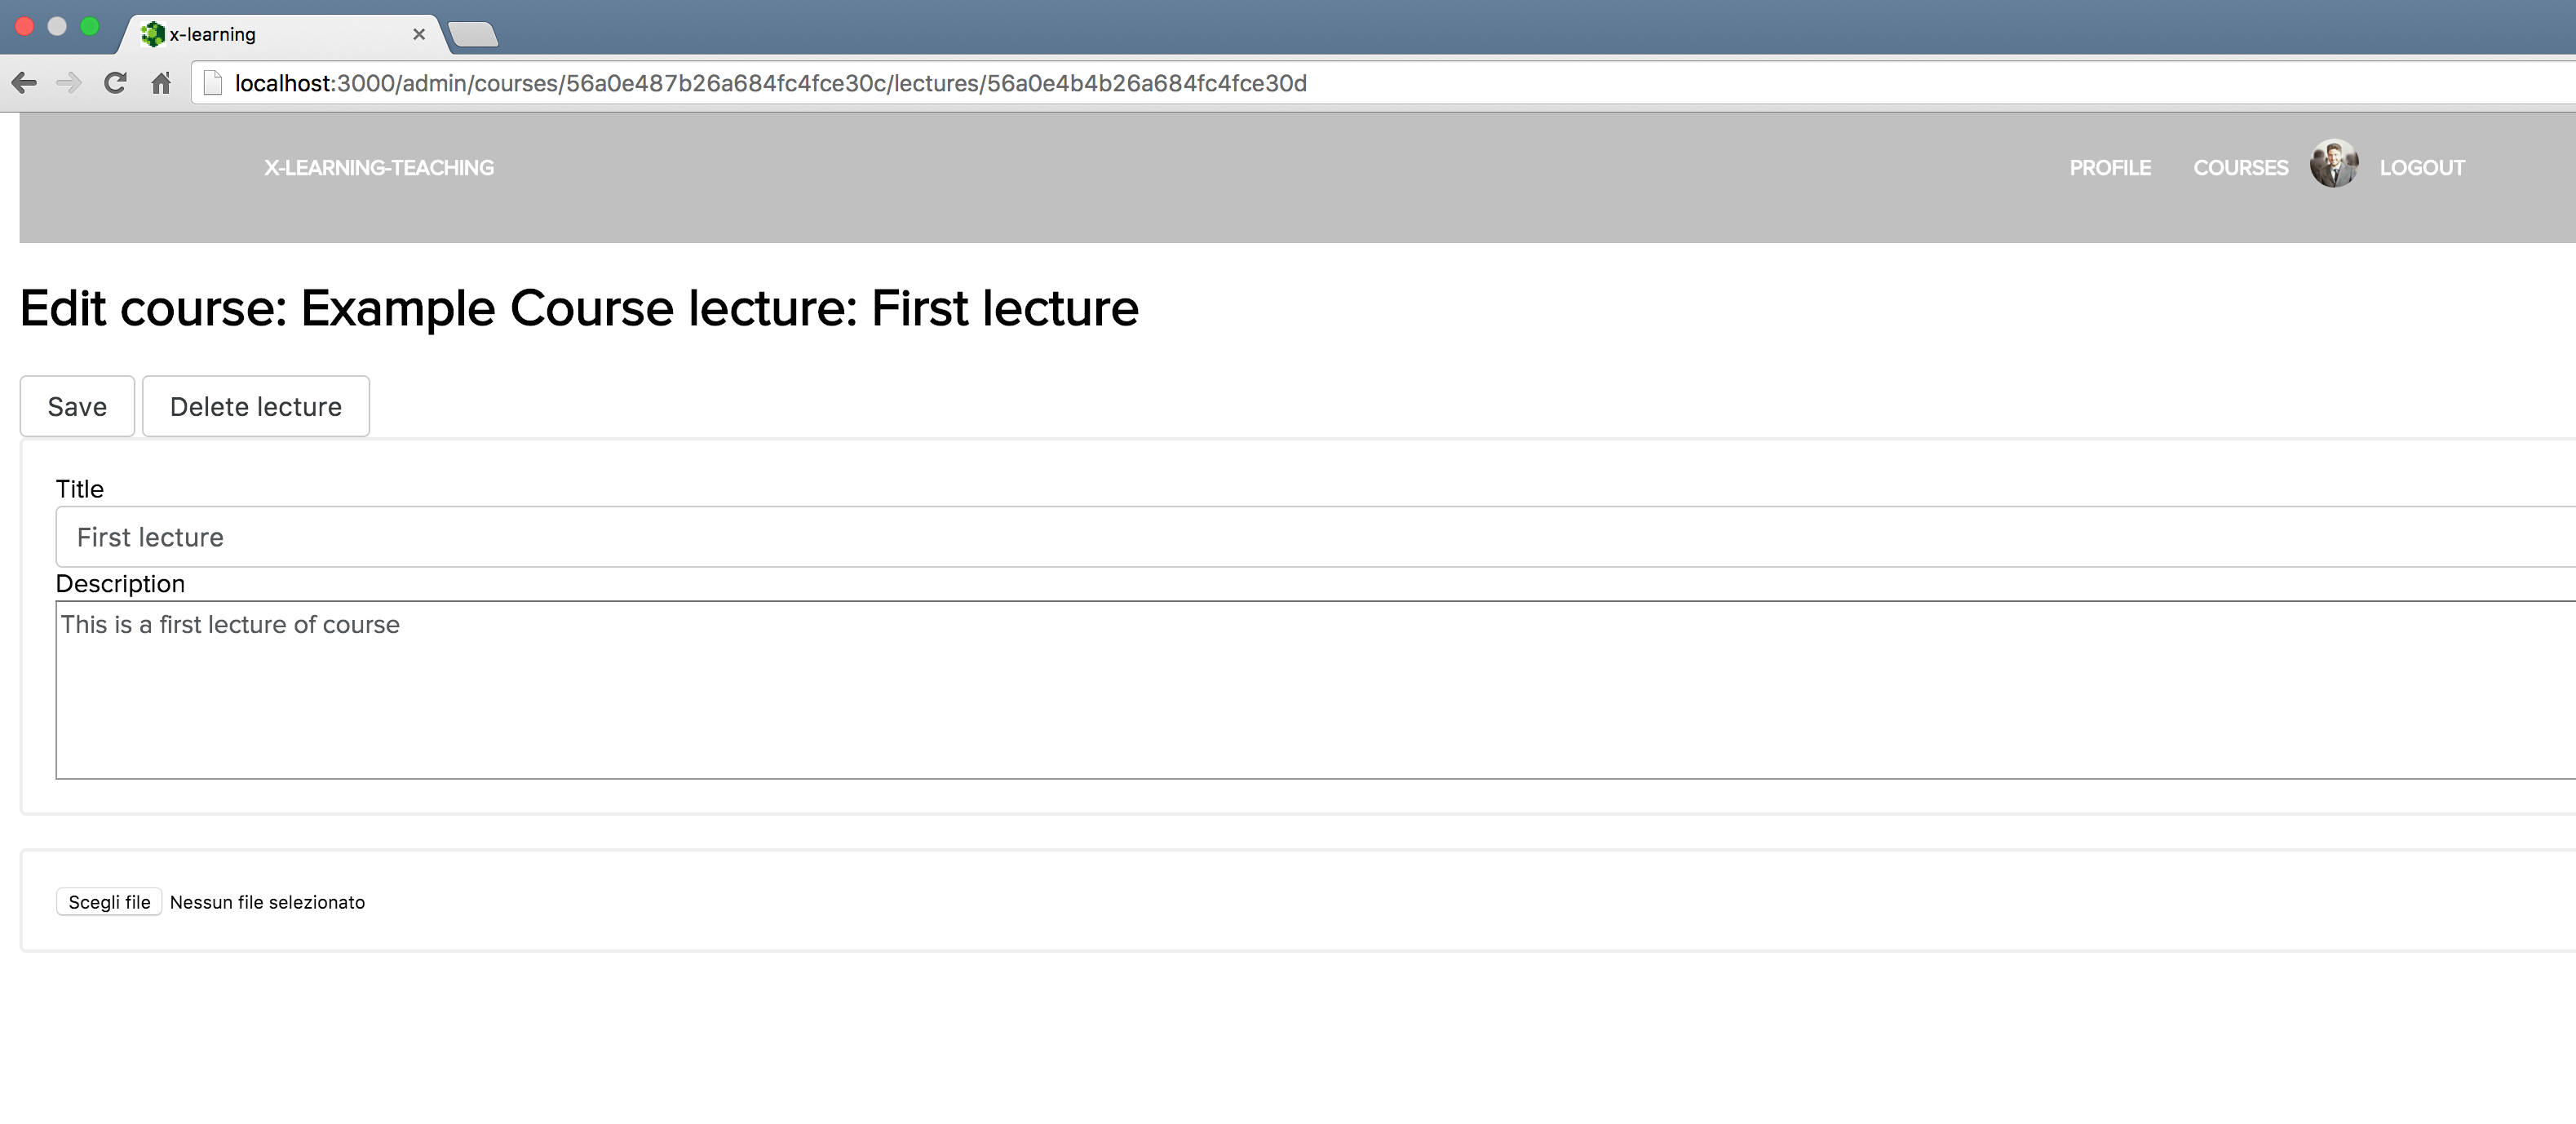
\includegraphics[width=1.0\linewidth]{images/chapter6/insert_lecture.png}\hfill
 \caption[Admin page lecture]{Admin page lecture}
 \label{fig:fourV}
\end{figure}

\end{itemize}

In order to allow the upload of the video on client side the following web component has been created:

\begin{lstlisting}[language=html]
      <input-s3-video></input-s3-video>
\end{lstlisting}

The following tag is responsible for the overall management of video uploading and transcoding. Furthurmore this component allows you to enter the video upload on any part of the project, hiding the full complexity that will be clarified in the following paragraphs.
A web component has also been created for streaming which allows video vision, hiding all encountered problems during the thesis and complexity that is shown in chapter 3.

\begin{lstlisting}[language=html]
       <deck-video src="{{data.lecture.video.url}}"></deck-video>
\end{lstlisting}